\subsection{Acteurs majeurs :}
Le développement des réseaux intelligents nécessite le concours  de nombreux acteurs :

\begin{itemize}[label=\textbullet]
\item \textbf{Les consommateurs:} en régulant eux-mêmes leur consommation d’électricité, participent à l’efficacité du système.

\item \textbf{Les producteurs d’électricité:} comme Sonalagaz en Algérie ou alors EDF en France alimentent les réseaux de transport  d’électricité et doivent être capables de répondre en temps réel à la demande. Le développement des smart grids permet également aux producteurs décentralisés de petites capacités (ex : les éoliennes ou les panneaux photovoltaïques appartenant à des particuliers) d’être raccordés.

\item \textbf{Les gestionnaires des réseaux de transport et de distribution ainsi que les constructeurs de matériel électrique} qui gèrent et installent les équipements de mesure assurant la sécurité et le fonctionnement des réseaux Ils sont les acteurs techniques majeurs du développement des smart grids.

\item \textbf{Les gestionnaires de processeurs et de systèmes informatiques:} comme InfoVista, Intel, Google ou Cisco System, développent les technologies d’information indispensables au fonctionnement des réseaux intelligents.

\item \textbf{Les pouvoirs publics:} soutiennent et encadrent le développement des réseaux intelligents notamment par la d1éfinition de normes de communication et la protection des systèmes contre les intrusions ou détournements.
\end{itemize}

\begin{figure}[h]
	\centering
    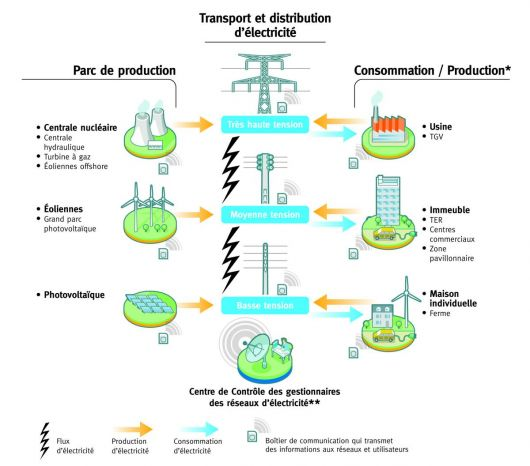
\includegraphics[scale=0.6]{img/part2/1.3}
    \caption{Intervention des acteurs dans le fonctionnement du Smart Grid.}
\end{figure}